\chapter{Raziskovanje podatkov}
\label{ch:raziskovanje-podatkov}

\newthought{Sedaj bomo zakopali globoko v podatke} in pogledali, ali se v njih skriva kaj zanimivega. Najlažji način, da spoznamo podatke, je, da jih prikažemo v grafih. \widget{Box Plot} (škatla z brki) nam pomaga odkriti osamelce, porazdelitve in zanimive spremenljivke.

Poglejmo, ali nam Box Plot pove kaj zanimivega. Namig: poiščimo razlike med spoloma. Te so vedno zanimive in občasno celo resnične.

\begin{figure}[h]
    \centering
    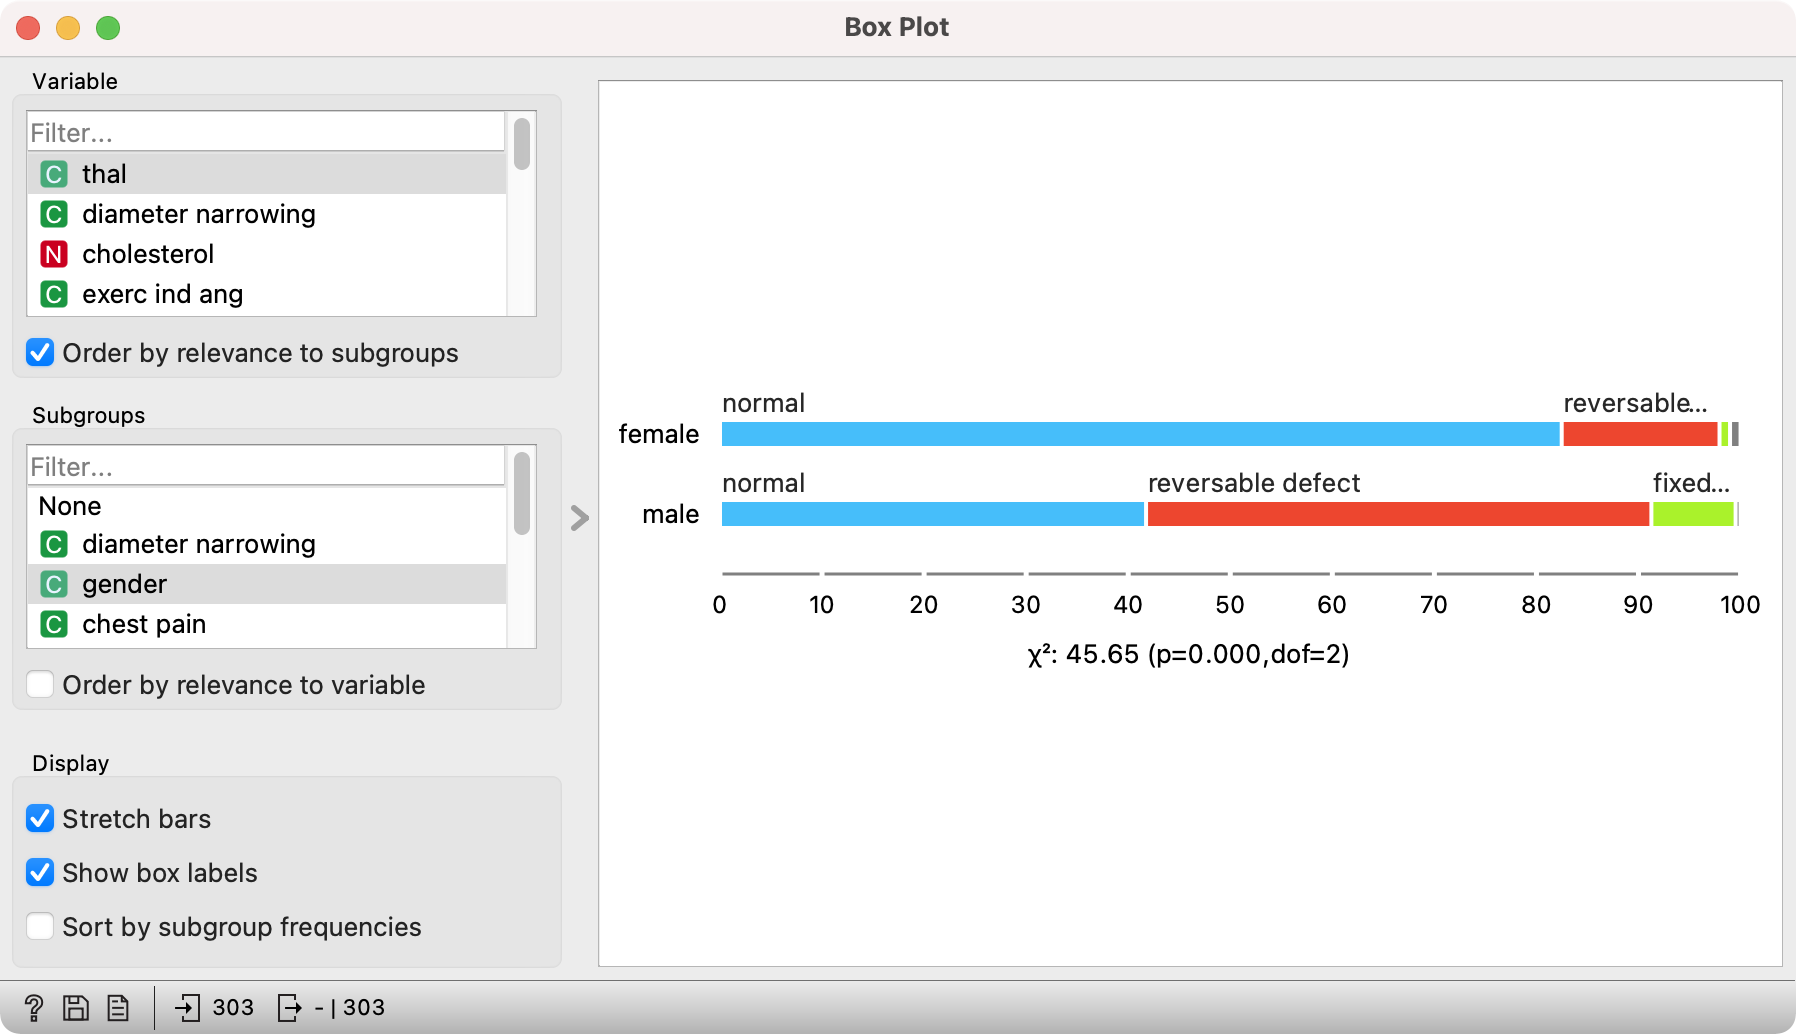
\includegraphics[width=\textwidth]{box-plot.png}
    \caption{$\;$}  % empty caption for correct figure placement
\end{figure}

\begin{wrapfigure}{o}{0.95\textwidth}
    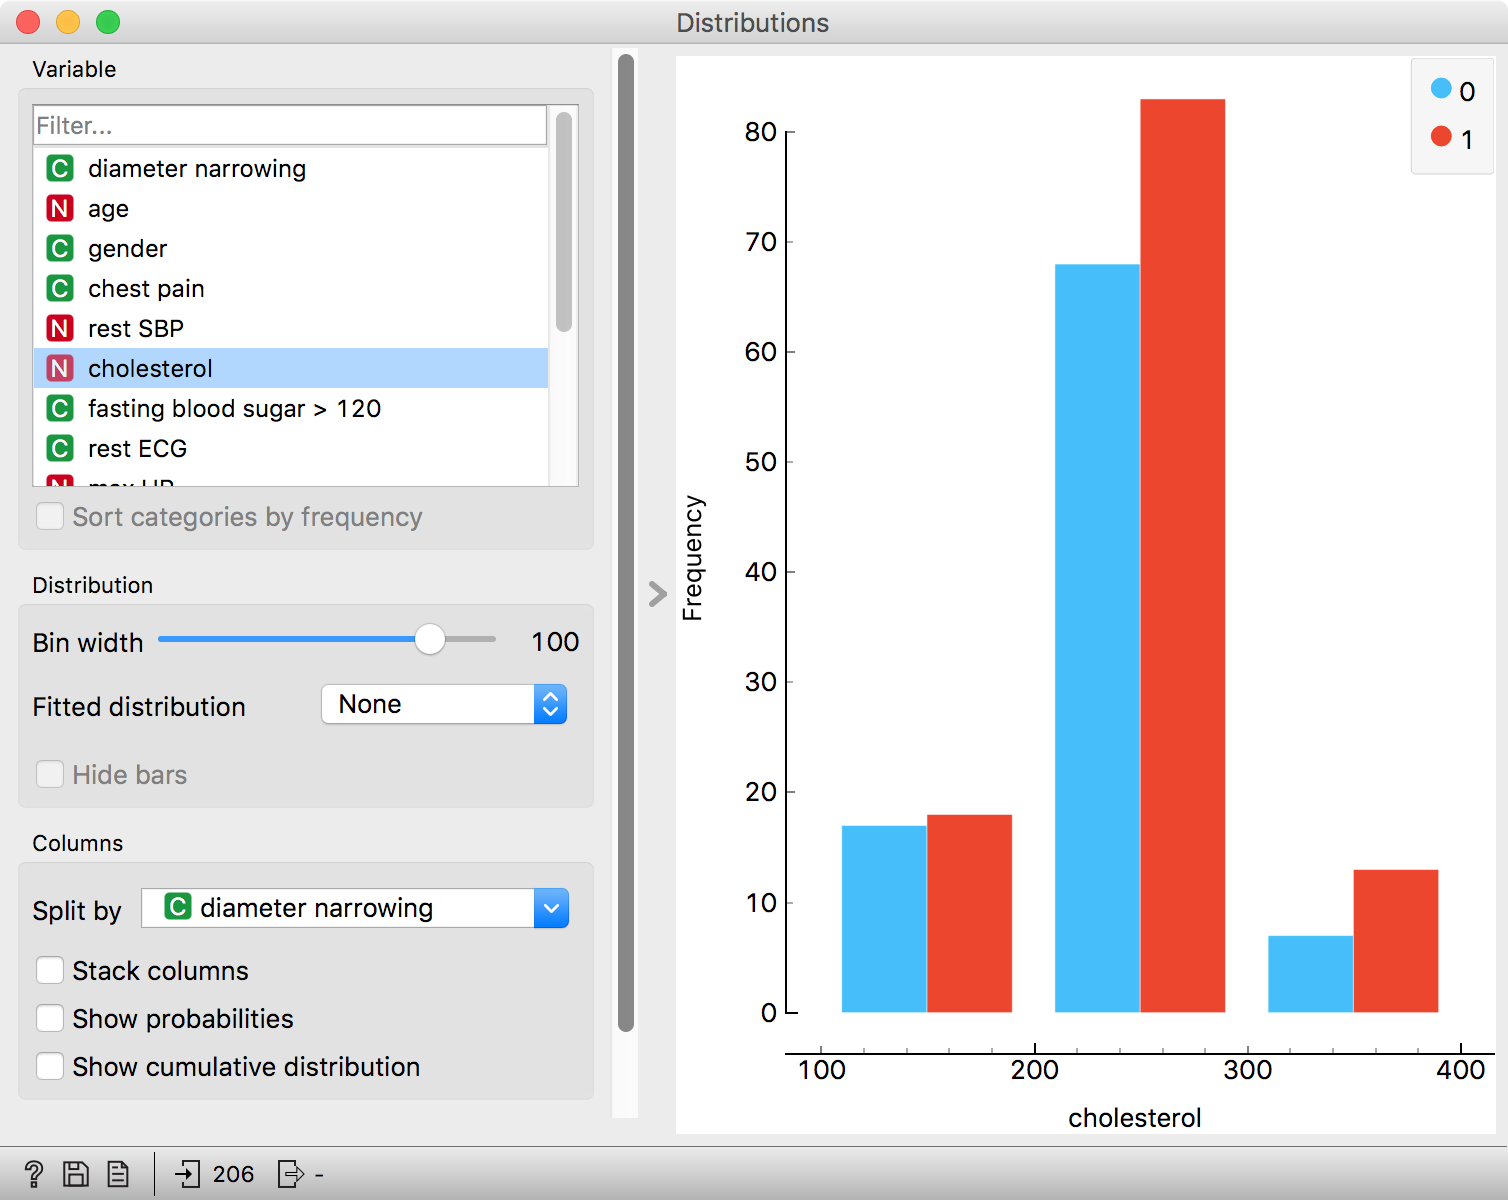
\includegraphics[scale=0.35]{distributions.png}
    \caption{$\;$}
\end{wrapfigure}

V razdelku \textit{Subgroups} smo podatke razdelili po spolu (gender) in nato odkljukali opcijo ‘Order by relevance’, ki spremenljivke razvrsti po tem, kako dobro ločijo med podskupinami. Moški v podatkih imajo slabše rezultate testa s talijem kot ženske.
Poglejmo si še gradnik \widget{Distributions}, ki je precej podoben Box Plotu. Prikazuje nam porazdelitve spremenljivk. Kakšna je porazdelitev starosti pacientov?

Podatke lahko razdelimo tudi po eni od spremenljivk  — v našem primeru po spolu — in jih pregledamo ločeno.

\newpage
\clearpage

V gradniku \widget{Select Rows} izberemo moške paciente (gender is male), dodamo pa lahko še dodatne pogoje. Izbira podmnožic odlično deluje z vizualizacijami porazdelitev. Odprite oba gradnika hkrati in preiščite podatke.

\marginnote{Gradnika Distributions dobita različne podatke: zgornji dobi izbrane vrstice, spodnji pa preostale. Z dvojnim klikom na črto med gradniki lahko povezavo uredimo in Orangeu povemo, da želimo v spodnji gradnik poslati preostale podatke.}

\begin{figure}[h]
    \centering
    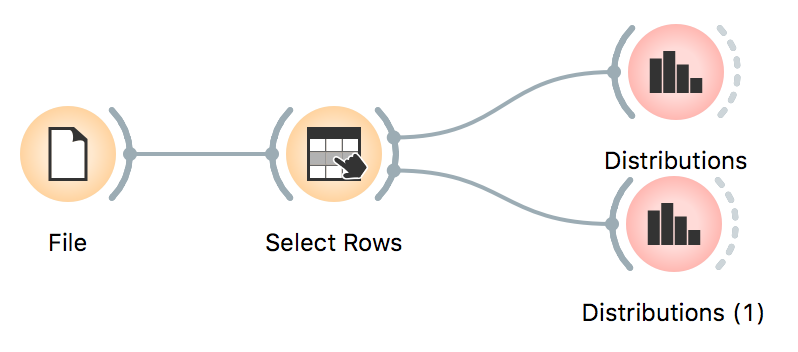
\includegraphics[width=0.9\textwidth]{select-rows-workflow.png}
    \caption{$\;$}  % empty caption for correct figure placement
\end{figure}

Tako Box Plot kot Distributions prikazujeta eno samo spremenljivko. Obstajajo pa tudi vizualizacije, ki lahko prikažejo več spremenljivk hkrati, tako da lahko vidimo povezave med njimi.

\begin{figure*}[h]
    \centering
    \newcommand{\wf}{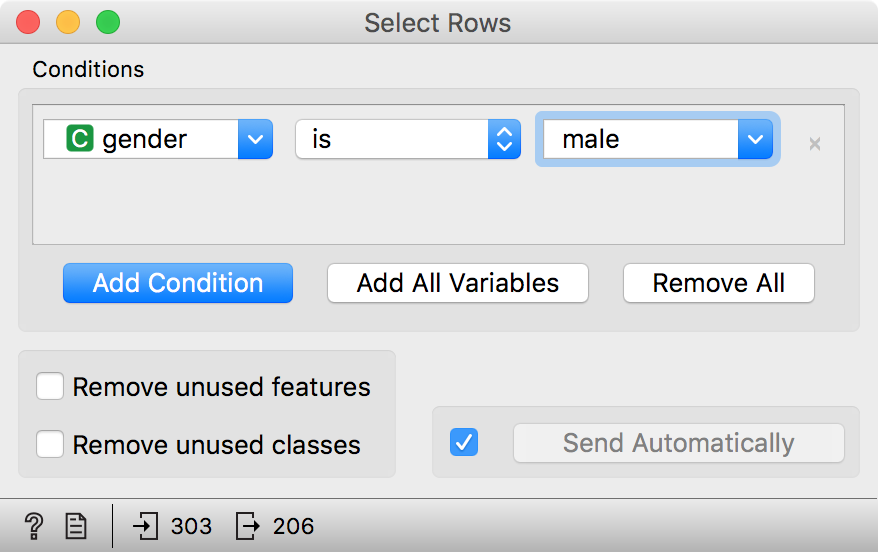
\includegraphics[scale=0.5]{select-rows.png}}
    \newcommand{\distrib}{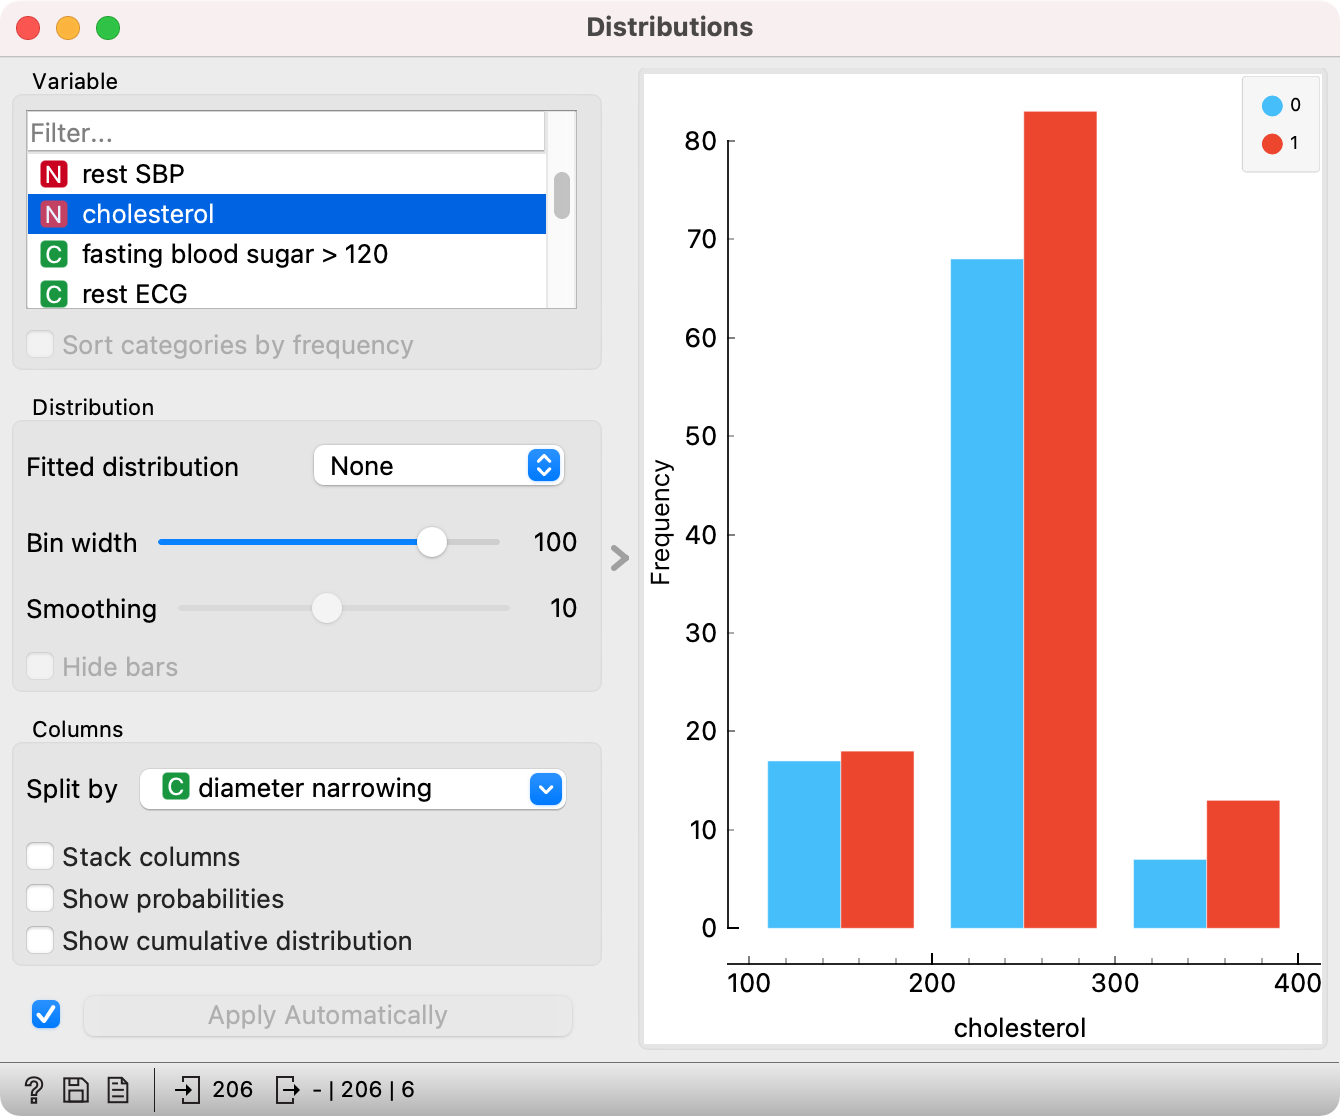
\includegraphics[scale=0.45]{distributions-subset.png}}
    \infinitewidthbox{
    \stackinset{r}{-0.5\linewidth}{t}{+0.2\linewidth}{\distrib}{\wf}\hspace{8cm}
    }
\end{figure*}

\newpage

\begin{figure}[h]
    \centering
    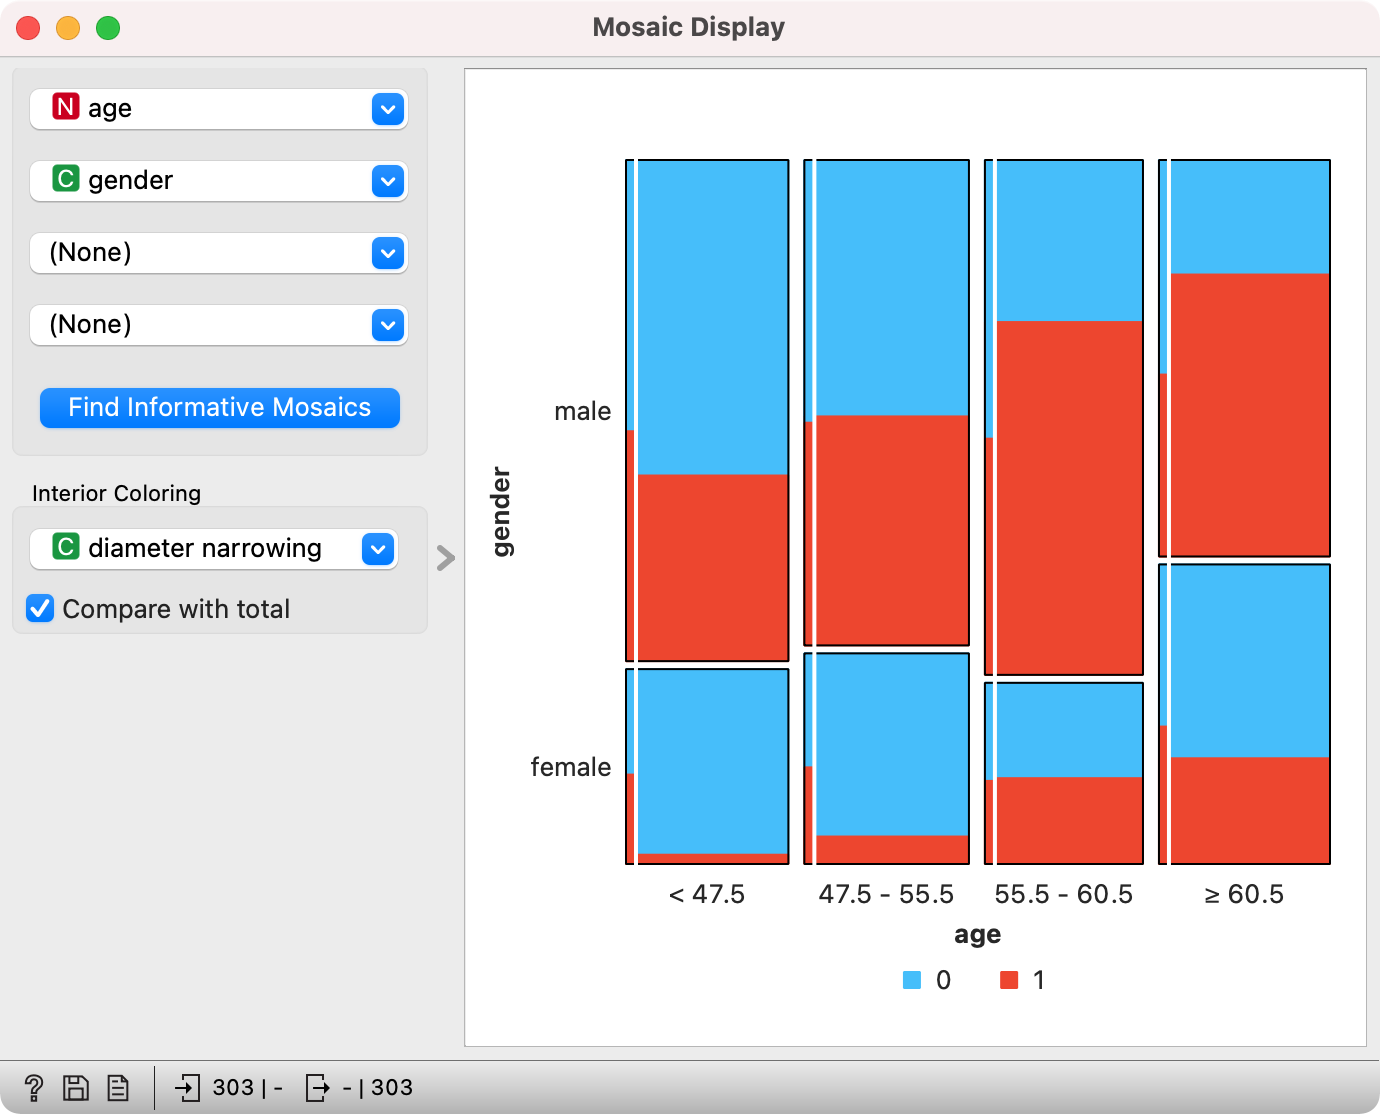
\includegraphics[width=0.95\textwidth]{mosaic-display.png}
    \caption{$\;$}  % empty caption for correct figure placement
\end{figure}

\marginnote{V gradniku lahko nastavite vizualizacije od ene do štirih spremenljivk. Preglejte različne vizualizacije.}\widget{Mosaic Display} prikaže pravokotno razrezane stolpce, kjer je širina pravokotnika sorazmerna s pogostostjo različnih tipov bolečine v prsih. Vsak stolpec se nato naprej deli vertikalno po starosti. Pravokotniki se lahko delijo naprej še po spolu (y os). Znotraj pravokotnikov nam rdeča in modra polja pokažejo porazdelitev ciljne spremenljivke za podskupino, tanke črte ob strani pa prikažejo splošno porazdelitev.

Kaj lahko razberemo iz tega diagrama?

\begin{wrapfigure}{o}{0.95\textwidth}
    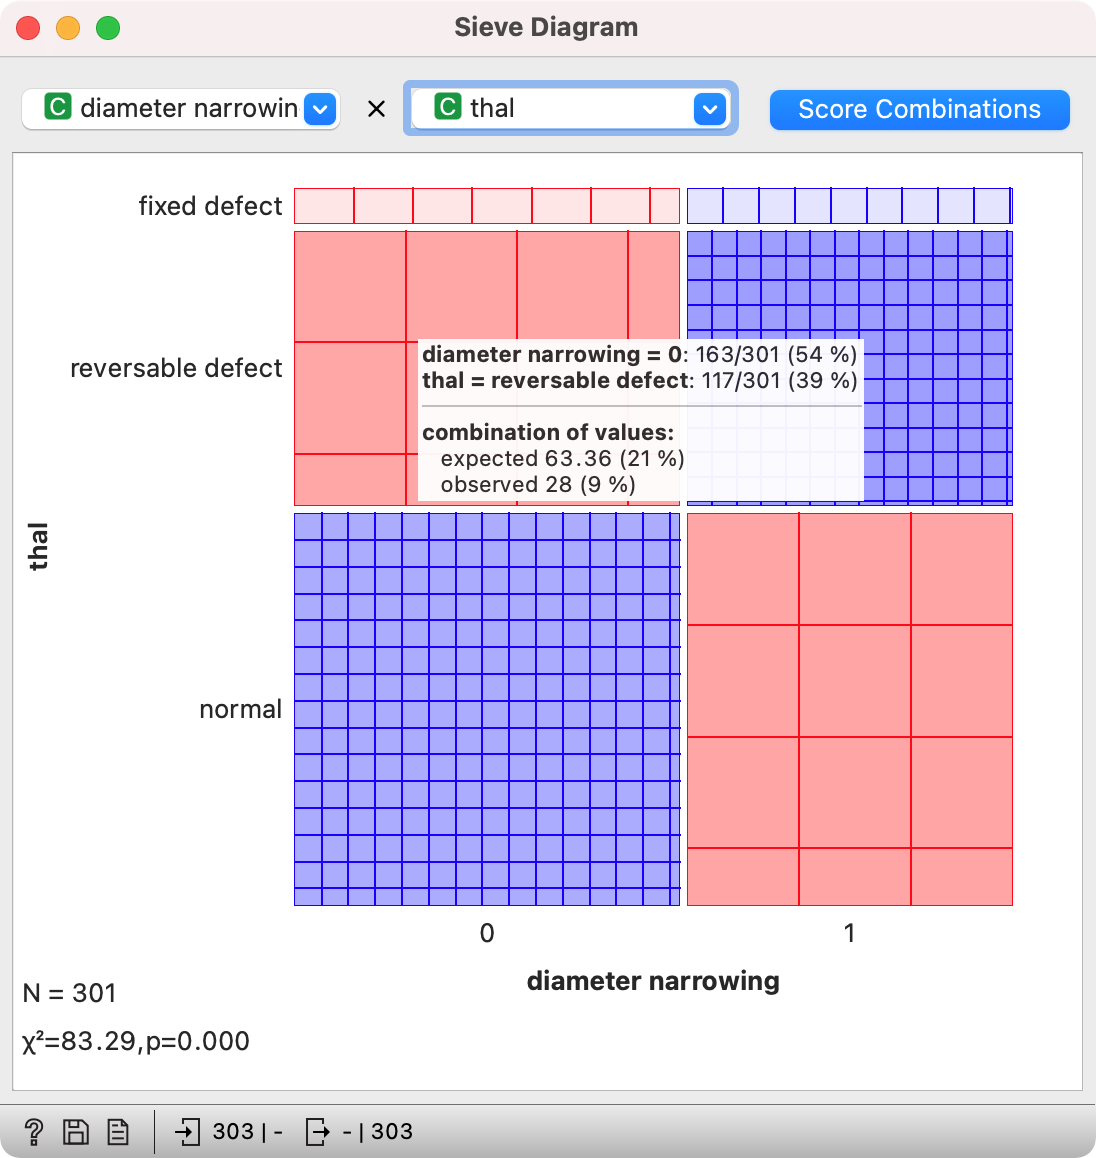
\includegraphics[scale=0.5]{sieve-diagram.png}
    \caption{$\;$}
\end{wrapfigure}

\widget{Sieve Diagram} takisto vodoravno in navpično deli pravokotnik, ki predstavlja množico pacientov, le da so rezi neodvisni, tako da je površina pravokotnika sorazmerna s pričakovanim številom pacientov, če predpostavimo, da so opazovane spremenljivke neodvisne. Npr.  1/2 pacientov nima srčne bolezni in 2/5 pacientov ima zaznano reverzibilno okvaro na testu s talijem. To pomeni, da je označen kvadrat velik 1/5 celotne površine. Od približno 300 pacientov iz celotne zbirke bi v tem delu pravokotnika pričakovali 1/5 × 300 = 60 pacientov, ki nimajo srčne bolezni in imajo reverzibilno okvaro. Vendar je teh le 28. Ta kombinacija je torej redkejša, kot bi pričakovali. Sievov diagram tako kaže razliko med pričakovano in dejansko verjetnostjo z gostoto mreže in barvo polja.